\section{Overall Description}
\subsection{Perspective}
Dream is a public domain, data aggregation platform and a knowledge network that provides all the functionalities described in section \textit{Product Functions (\ref{sec:product-function})}.\\
It exploits an IdP to supply authentication and authorization in all its components, that can be easily integrated with standard external services and it also takes advantage of API interfaces to retrieve data needed for the elaboration.

\subsubsection{User Interfaces}
The system should interface with different actors through devices which must be connected to Internet. The interfaces are provided via web application, which is responsive and can be used from different type of devices (e.g. desktop and tablet). Server side 

\subsubsection{Software Interfaces}
The system allows the Administrator to dynamically add external APIs in order to retrieve data needed for the elaboration.

\begin{figure}[h!]
    \centering
    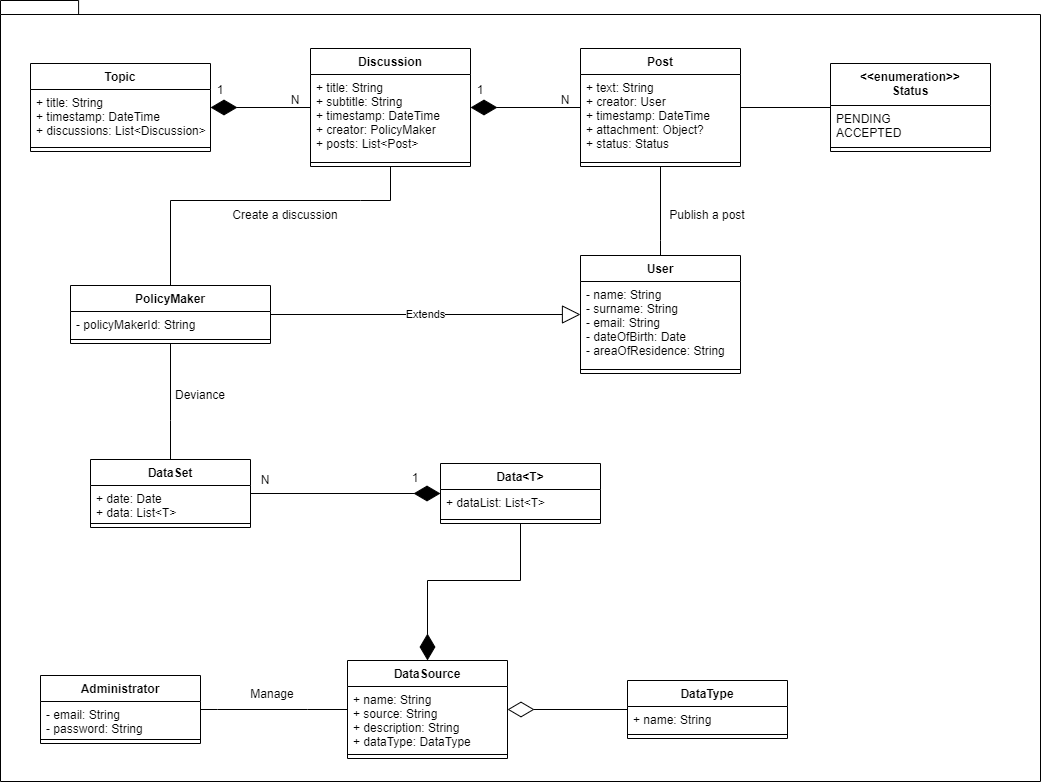
\includegraphics[scale=0.35]{images/class_diagram.png}
    \caption{Class diagram}
    \label{fig:class_diagram}
\end{figure}
\FloatBarrier

\subsubsection{Hardware Constraints} \label{sec:hardware_constraint}
Every person that wants to access the Dream service needs to have a device that features a browser and with an internet connection. Moreover the system is composed by a data-aggregator, on server side, that should have a stable and high speed internet connection (e.g. optic fiber).

\subsection{Product Function} \label{sec:product-function}
In this section are described only the bigger functions present in out system.
\subsubsection{Sign Up}
This functionality allows a Visitor to register in order to write in the Dream’s forum.
The first step is to insert all the requested credentials. If they are valid the system will send an email to the inserted address, asking the User to click on a link, in order to validate its account. At the end of the process the new User is taken to the login page.
\begin{figure}[h!]
    \centering
    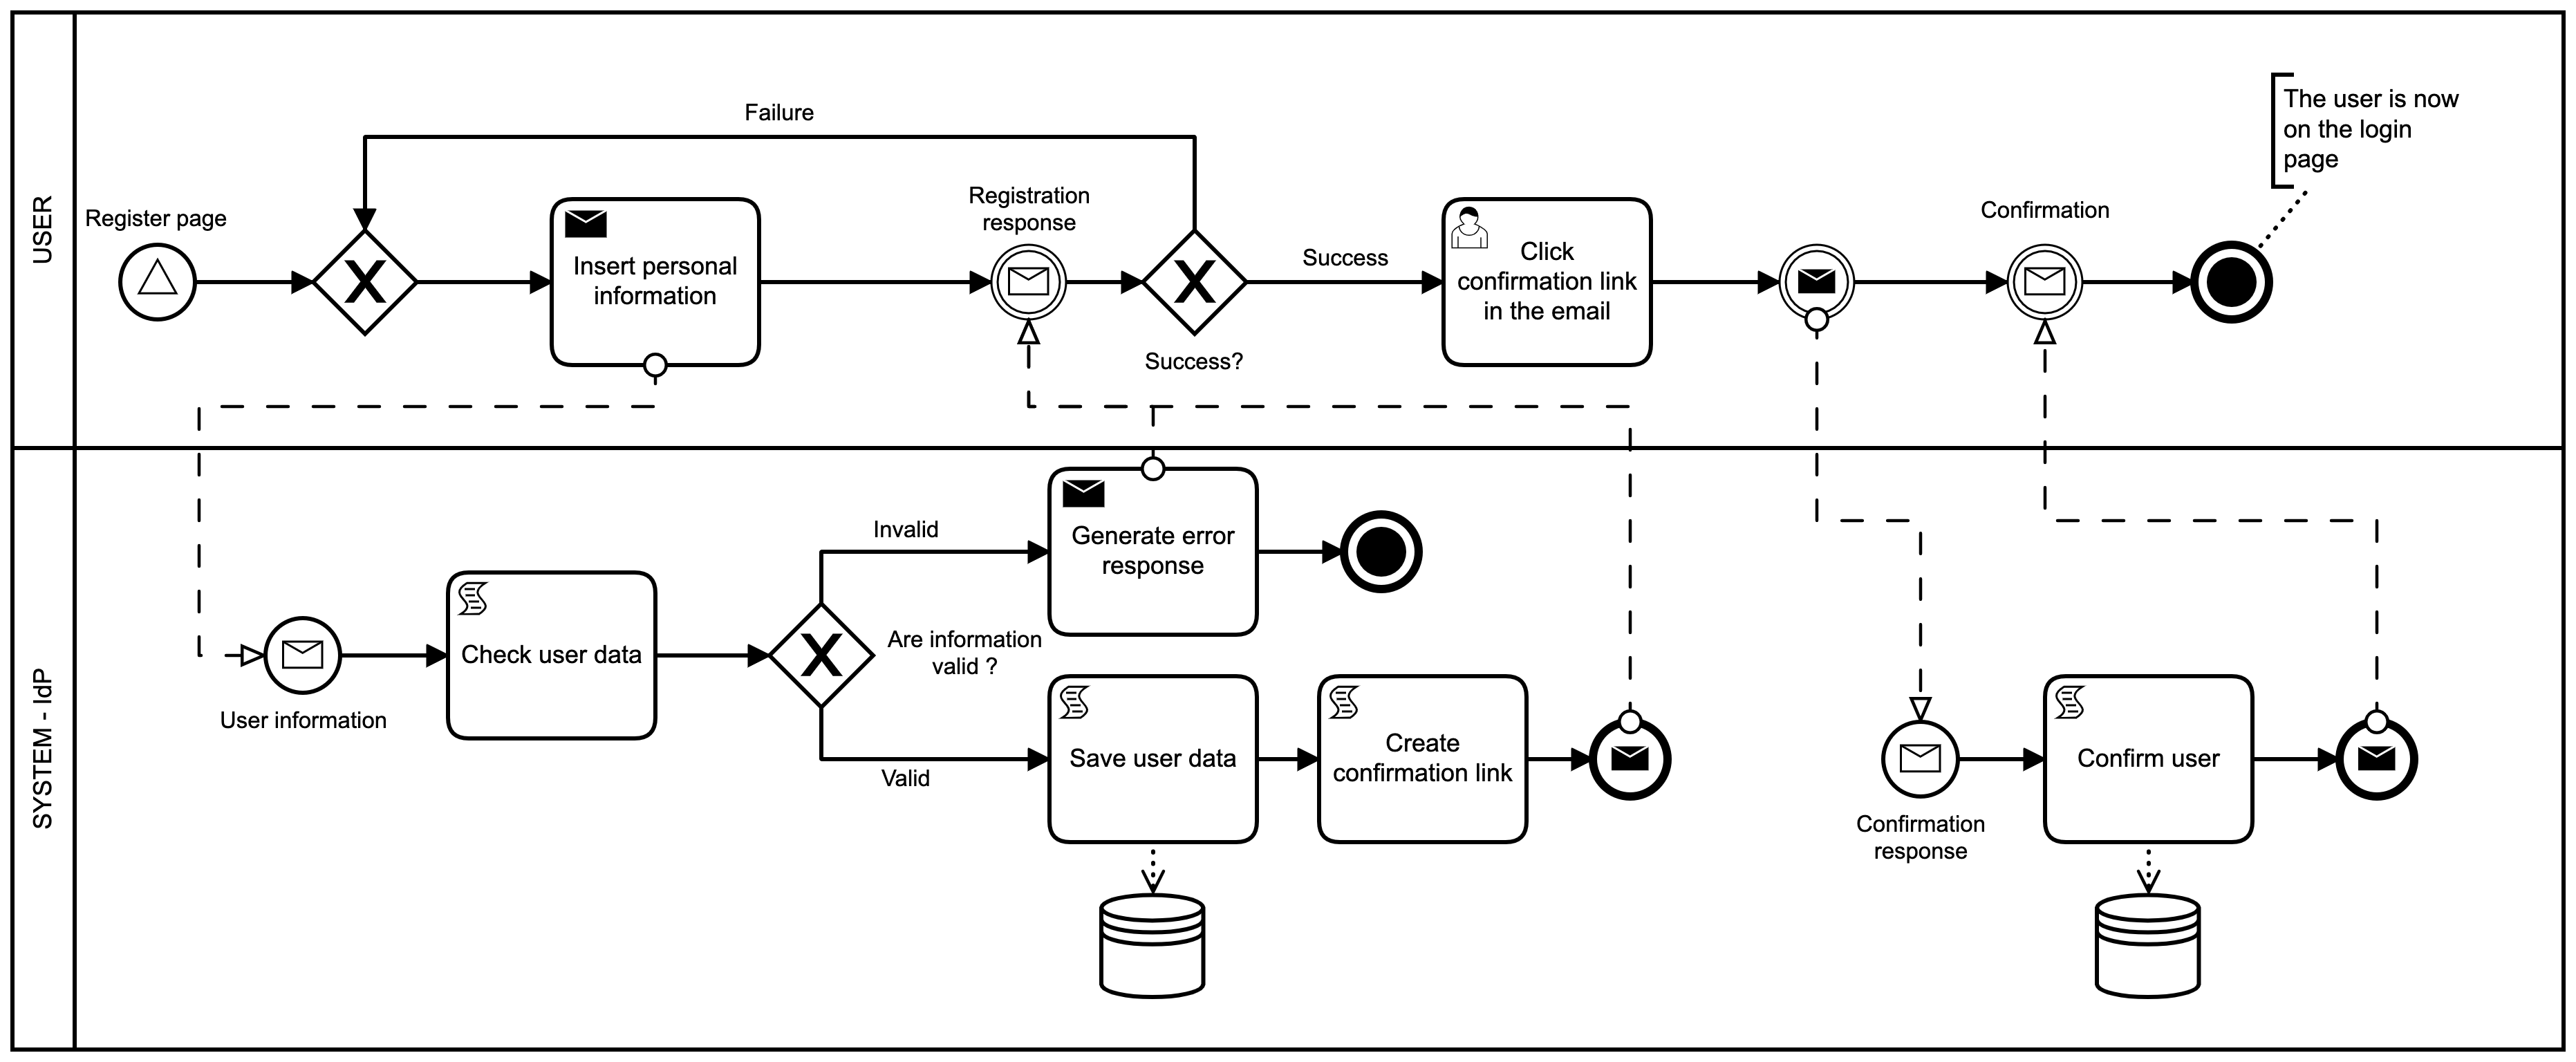
\includegraphics[scale=0.10]{images/bpmn/signup_bpmn.png}
    \caption{Sign Up BPMN}
    \label{fig:bpmn_signup}
\end{figure}
\FloatBarrier
\subsubsection{Deviance}
This functionality is accessible only to the Policy makers. By default the Deviance is going to be calculated by the system itself, according to predefined parameters. The Policy maker has the capability to make the system recalculate the Deviance, modifying the considered parameters. To do so he should go to his reserved area and click on the Deviance button, after that, he can select the different parameters from a list and then recalculates the Deviance.

\begin{figure}[h!]
    \centering
    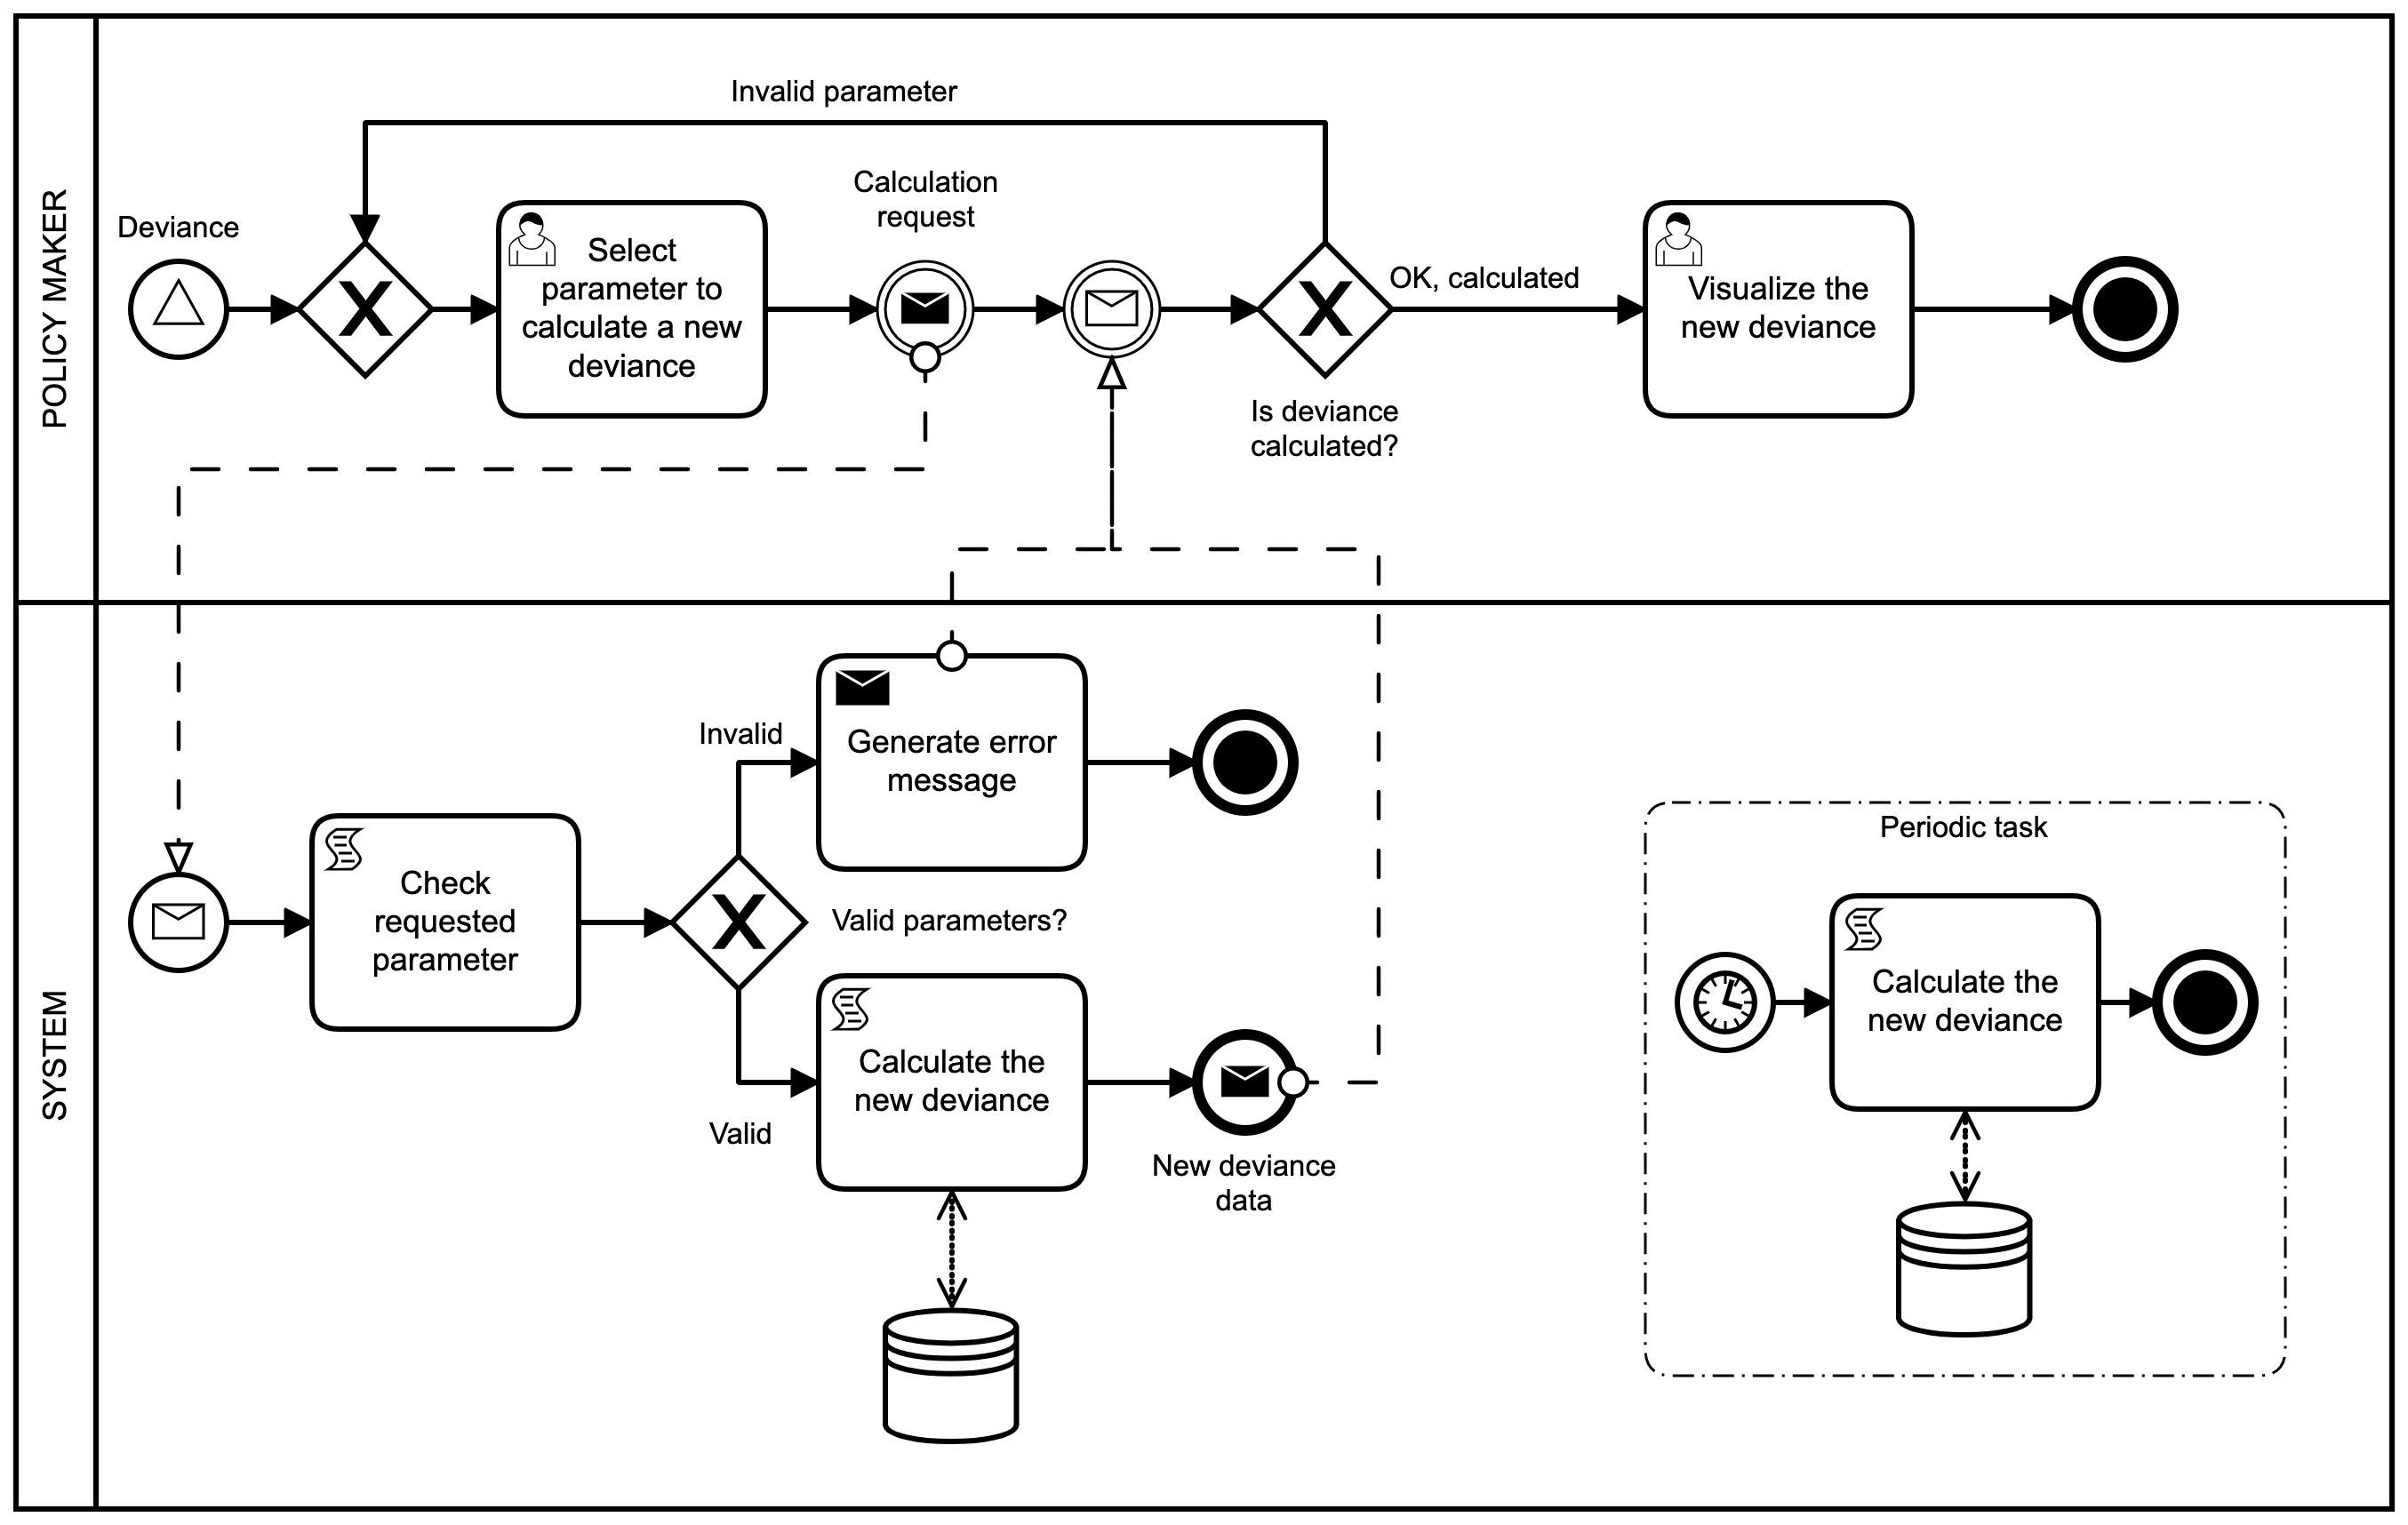
\includegraphics[scale=0.14]{images/bpmn/deviance_bpmn.png}
    \caption{Deviance BPMN}
    \label{fig:bpmn_deviance}
\end{figure}
\FloatBarrier

\subsubsection{Notification}
This functionality lets the system send a notification to a User when his post gets accepted or rejected by a Moderator. Also, a notification is sent when a new post is published in a discussion in which an User or Policy maker has interacted with.

\begin{figure}[h!]
    \centering
    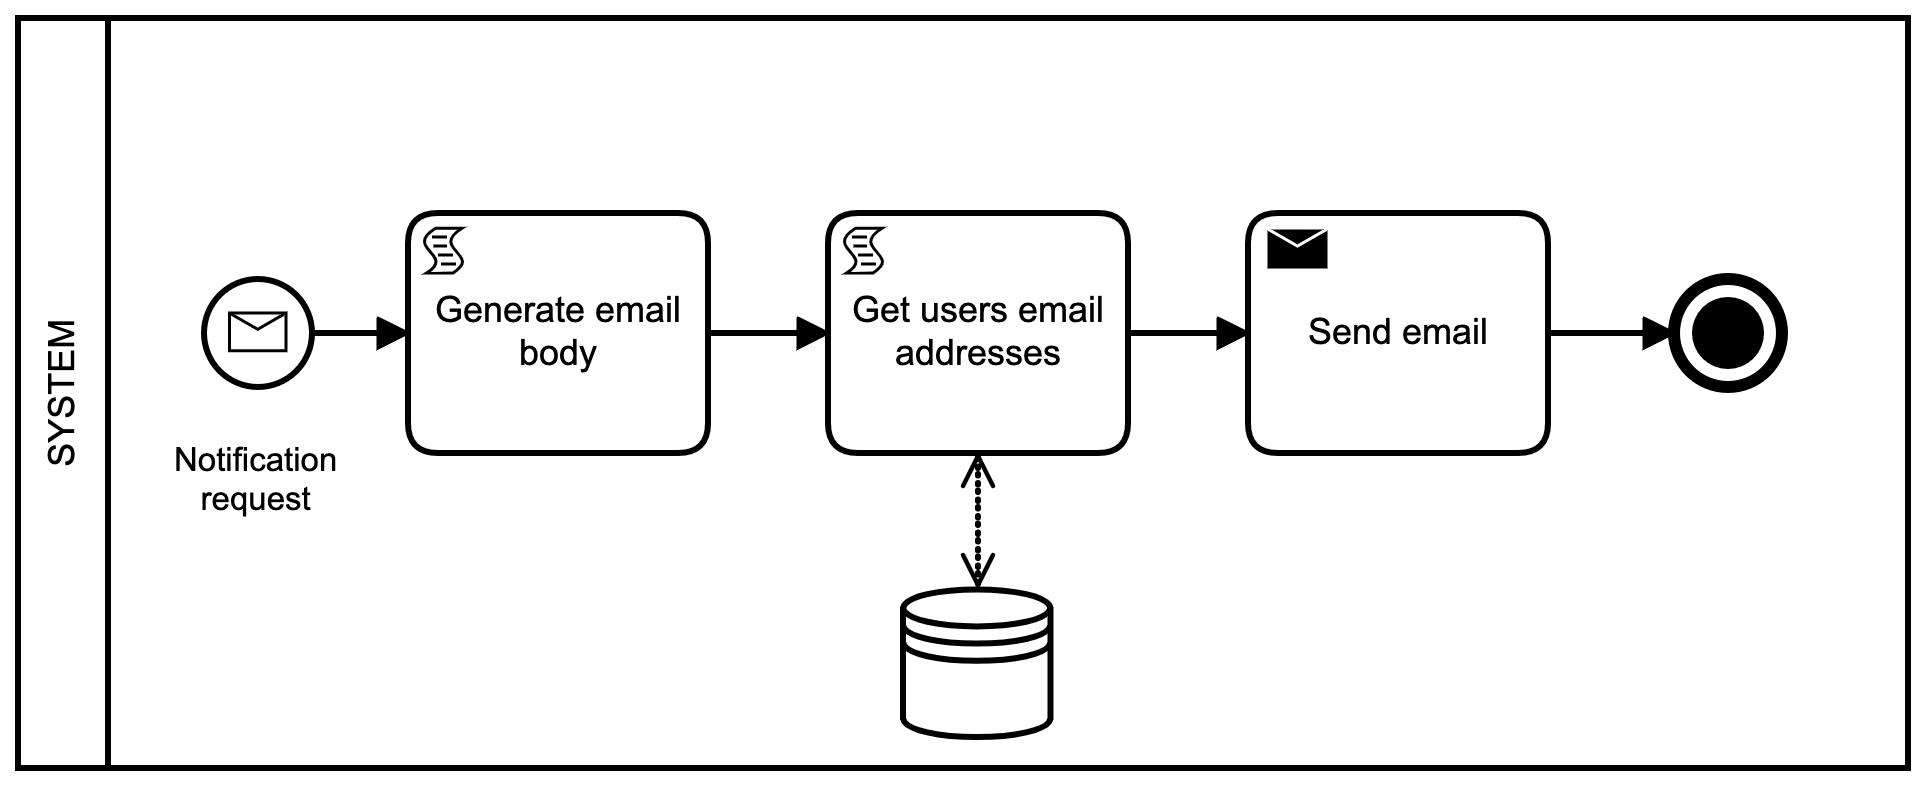
\includegraphics[scale=0.18]{images/bpmn/notification_bpmn.png}
    \caption{Notification BPMN}
    \label{fig:bpmn_notification}
\end{figure}
\FloatBarrier

\subsection{Actors}
\subsubsection{Visitor}
Whoever has accessed the site, without having an account. He can freely access the data, filter them, download them and he can also visit the forum and read all the discussions in it. The only limitation he has is that he can’t write in the forum.

\subsubsection{User}
A Visitor that has registered to the site and is logged in. In addition to all the functions of the Visitor he can also write replies in the forum.

\subsubsection{Policy maker}
A person who is in charge of building up the knowledge network, according to a ranking list. He can register to the site only if he owns a unique identifier (the Policy maker ID), that associates his real identity to the digital one. He can retrieve the ranking list (and also “forge” another one) in his private area.
In addition every Policy maker has the role of moderator in the forum.

\subsubsection{Administrator}
The administrator of the Dream’s site. He is the one who manages the data sources.

\subsection{Assumptions, Dependencies}
\subsubsection{Assumptions}
\begin{itemize}
    \item \textbf{D1:} The registration of a User in the IdP doesn’t imply the User registration in the SP.
    \item \textbf{D2:} The roles used by SPs are already correctly mapped by the IdP. 
    \item \textbf{D3:} A new discussion can be created only by a Policy maker.
    \item \textbf{D4:} Users can modify only their posts.
    \item \textbf{D5:} Policy makers are forum moderators.
    \item \textbf{D6:} Policy makers can modify all the posts.
    \item \textbf{D7:} The administration role could be given only by another Administrator.
    \item \textbf{D8:} The Policy maker ID is given by third parties.
\end{itemize} 

\subsubsection{Dependencies}
Administrator's accounts are the only ones who can manage the system. They can be created only from another Administrator, so an internal service is sufficient to manage this group of accounts.\\
Different types of User will access the forum, with different permissions and roles. For this reason it will be a good choice letting Users register in other identity providers to login using their already existing account so, an external authentication system is required. Meanwhile, Policy makers are internal user too but they can also interact with the forum. For that reason, it is also needed that the system act like an Identity Provider and, at this point, Users can register using the same IdP that Policy maker relies on.\\
Shibboleth is the most used service in academic field. It is structured to base the authentication process using a LDAP directory. For this reason, the user data needs to be saved in OpenLDAP. LDAP presents specific application to manage directory content and it relies on its own internal administrator.\\
This technology has to be considered as an external component in the project due to the fact that could also be used as a service in the cloud. 
